%************************************************
\chapter{All Things Classical}\label{chap:compilers}
%************************************************

Okay, maybe not \emph{all} things classical, but some things\dots
Okay, maybe just one or two really.

In this chapter we will give a very brief overview of the components of classical computers that will be helpful to further discussions of quantum circuit compilation.
A key component to quantum circuit compilation is the word ``compilation'' and its' origins (in computing) span back to the early 1950's when electronic digital computers were in their early stages.
Understanding the historical development of compilation and its' tecniques will provide ideas and tools necessary in solving the new task of quantum circuit compilation.

This chapter is meant to provide the reader with the basics of some computing terminology and ideas.
It is by no means a complete introduction to compilers, nor computer architecture.

\section{What can a computer do?}

If you're reading this, I'm sure you can imagine something your computer is capable of.
Maybe reading this document online, sending messages/email, browsing the internet, writing documents, etc.
These are very high level operations our computer can perform, but under the hood much more primitive operations are taking place.
It is these primitive operations that we wish to understand, and will have many similarities with modern-day quantum hardware.

A simplified model of computer architecture, known as the von Neumann Architecture (\cref{fig:comparch}) shows what we now call a \ac{CPU} which is the workhorse of the computer.\footnote{At least in this \emph{very simplified} model.}

\begin{figure}[h]
    \centering
    \includestandalone[width=0.8\textwidth]{tikz/arch}
    \caption{von Neumann Architecture scheme}\label{fig:comparch}
\end{figure}

Since the \ac{CPU} is the computational piece of a computer, what can it do?
Most modern \acp{CPU} are built on the \acp{ISA} which means that the \ac{CPU} has a finite set of operations or instructions that it can perform and everything we might wish to perform on a computer, must be built up from these primitive operations.
Some examples of what these primitive operations might be are
\begin{itemize}
    \item put a value into memory,
    \item add two values in memory together and store in a new location,
    \item perform the bitwise negation on a value,
    \item compute the square root of a value.
\end{itemize}
With a set of performable operations laid out, one can then use these primitives to build up more and more complex functionality that eventually implements the things we know and love (and hate) computers for.
One thing worth mentioning here that is often glossed over in treatments of \acp{ISA} is that the instruction set must be computationally universal.\footnote{Or Turing-complete if you're computer science oriented.}
Without going too much into the weeds, we should think of computationally universal (in the classical sense) as wielding the full power of a computer, rather than only being able to do a particular type of computation.\todo{I don't like this explanation.}
Thankfully, this is relatively easy to do in the classical setting and there are even theoretical machines that use a \emph{single} operation to achieve universal computation.
\Eg{} one can achieve universal classical computation with the following instruction which implements ``subtract and branch if negative''.
\begin{lstlisting}
    Instruction subneg a, b, c
    Memory[b] = Memory[b] - Memory[a]
    if (Memory[b] < 0)
        goto c
\end{lstlisting}

While this style of architecture is great, and has worked very well, it requires the programmer to code at a very low level since the operations a \ac{CPU} performs are themselves primitive.
In order to work at a higher level of abstraction, computer scientists and programmers began to create new languages which were easier to read and write, yet could be translated into a form the brains of the computer could understand.
This would improve productivity by allowing those writing code to work at a higher level of abstraction, and bury implementation details into the code which performed the translation into the machine's instruction set.
The software responsible for translating these higher level ideas into a machines instruction set are known as \textbf{compilers}.


% With the exception of the last item, these operations are generally considered to be simple, and the latter complex.
% This has given rise to a distinction in \ac{CPU} architecture where we see \acp{CISC} and \acp{RISC}.
% The goal of the former to implement more and more complex ``primitive'' operations, while the latter leaving more work to be performed by the compiler~\cite{dragonbook}.

\section{Compilers}

While compilers have their origins in the aforementioned translation of higher level code into lower level code, they have grown considerably to perform many more tasks.
Before we dive into all of the capabilities of a modern compilers, let's take a step back and recall what the word compile means.

Merriam-Webster defines the word \textbf{compile} to mean~\cite{compiledef}
\begin{quote}
    to compose out of materials from other documents.
\end{quote}
In this context we might imagine ``other documents'' to mean the higher level code (and maybe other configuration files) and we are composing the lower level machine code.
We can see this definition reflected in~\citetitle{dragonbook}\footnote{Colloquially known as ``The Dragon Book'' because of the cover, and likely the most famous book on (classical) compilers. This is also where the logo of the LLVM project originates from which we will discuss in~\cref{sec:llvm}.}\graffito{
    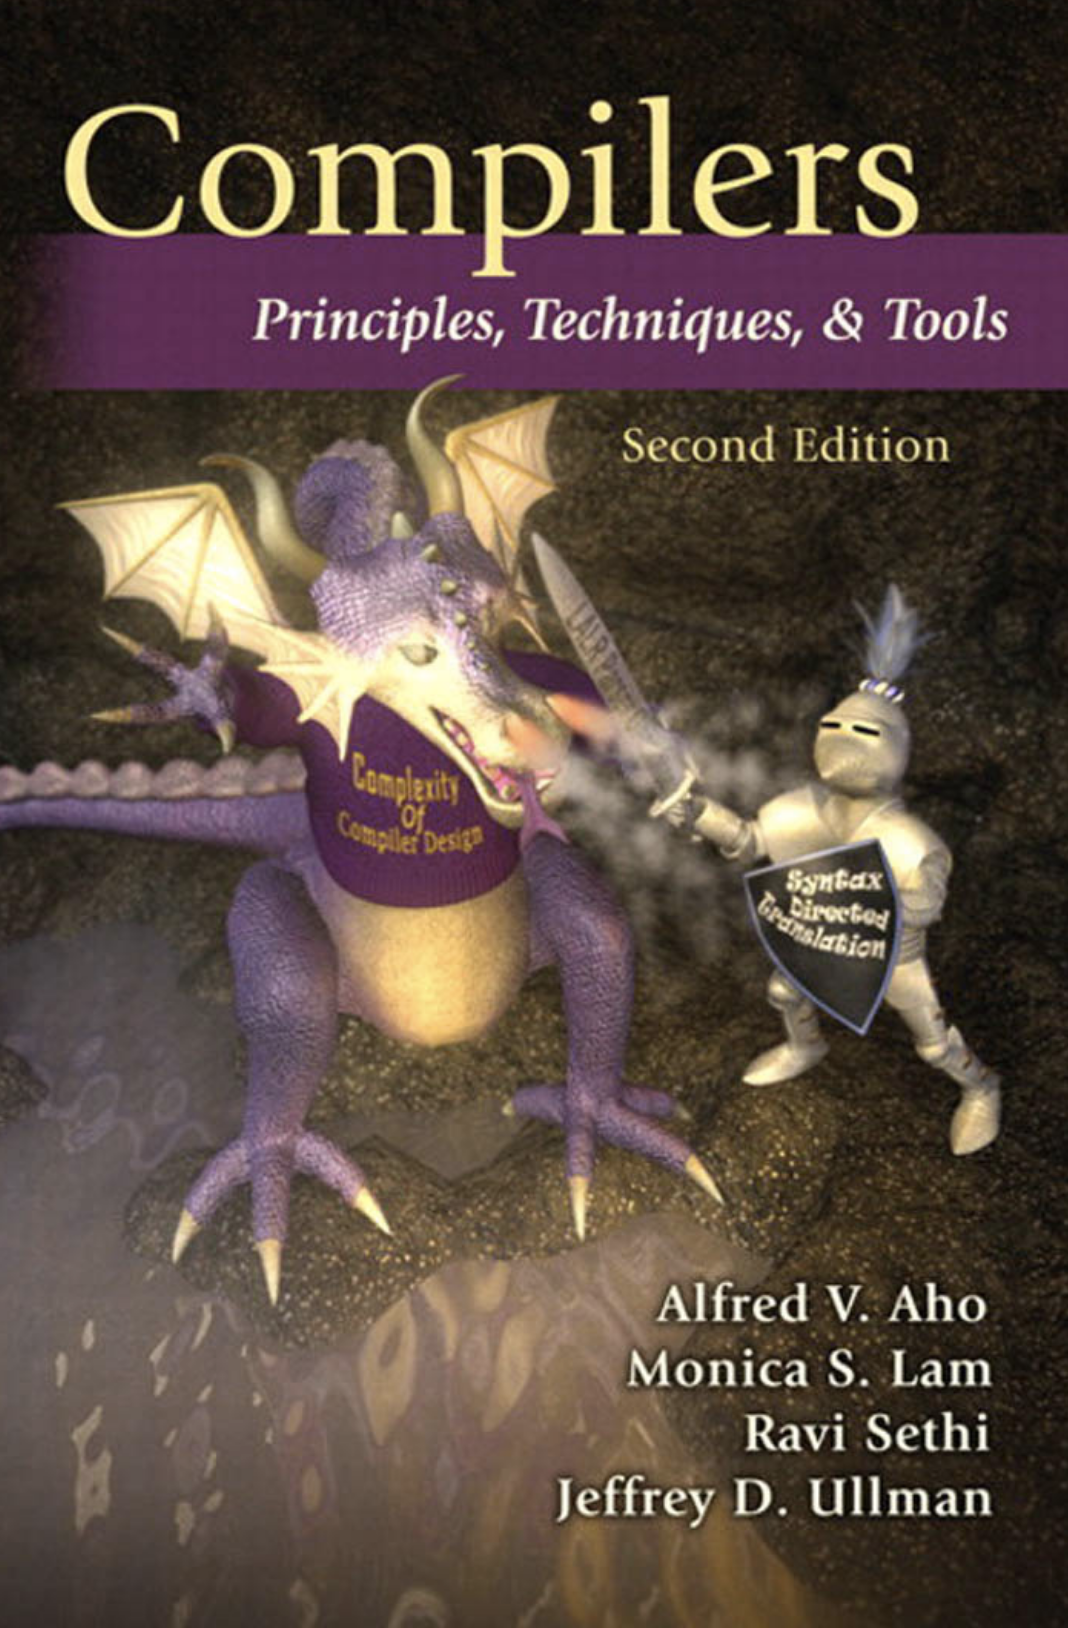
\includegraphics[width=\marginparwidth]{img/dragonbook.png}
    \emph{The Dragon Book}
    
\includegraphics[width=\marginparwidth]{img/llvmlogo.png}
    \emph{LLVM Logo}
}~\cite{dragonbook} where the authors introduce compilers through the process of transforming software.
\begin{quotation}
    [B]efore a program can be run, it first must be translated into a form in which it can be executed by a computer.

    The software systems that do this translation are called \emph{compilers}.
\end{quotation}
Hence we can view compilers as a function taking software written at one level of abstraction and bringing it down to a lower level that a computer's \ac{CPU} can understand.
\begin{figure}[ht]
    \centering
    \includestandalone[width=0.8\textwidth]{tikz/compiler}
    \caption{Action of Compiler}\label{fig:compiler}
\end{figure}

The term compiler was coined by Grace Hopper in the early 1950's while working on a system that could translate symbolic mathematics into a machine language.
Initially Hopper's new idea was met with resistance.
\begin{quotation}
    I had a running compiler, and nobody would touch it because, they carefully told me, computers could only do arithmetic; they could not do programs.
    It was a selling job to get people to try it.
    I think with any new idea, because people are allergic to change, you have to get out and sell the idea.
    \attrib{Grace Hopper 1952~\cite{hopperquote}}
\end{quotation}
In the end she succeeded in selling the idea and compilers became a ubiquitous piece of modern computing infrastructure.
Some of the many functions a modern compiler can perform are line reconstruction, preprocessing, lexical analysis, syntax analysis, semantic analysis, conversion to an \ac{IR}, optimization, and finally code generation.
Thankfully we will not need to understand all of these parts, and the majority of this document will focus on \aclp{IR}, optimizations, and code generation.

\subsection{Compilation Phases}

As alluded to in the previous section, a compiler has many different responsibilities.
Each responsibility is broken into a separate component so that it can be understood on it's own.
A schematic for this can be seen in~\cref{fig:compilerphases} for the main steps that we will be concerned with in this document.
\begin{wrapfigure}[24]{i}{0.25\textwidth}% TODO tweak lineheight
    \centering
    \includestandalone[width=0.23\textwidth]{tikz/phases}
    \caption{Compiler Phases}\label{fig:compilerphases}
\end{wrapfigure}

\paragraph{Syntax Analyzer}
This phase is for ensuring the code is syntactically well formed (that is it abides by the specification of the language).
If one is writing code in a binary alphabet with characters \texttt{0} and \texttt{1}, then the ``program'' \texttt{00011} is syntactically valid, while \texttt{1102} is not because a \texttt{2} appears in the code.
To complete this step many compilers turn the code into a syntax tree to complete the verification.

\paragraph{Semantic Analyzer}
During this step the program is validated in such a way that ensures the code can run on a computer.\todo{this is a bad description}
Part of this is usually doing type checking to ensure calculations are computed between valid types.
In many languages the operation \texttt{'hello' * 5} would pass the syntax analyzer, but fail the semantic analyzer because a string multiplied by an integer is usually not defined.\footnote{It is completely valid in other languages though like python!}

\paragraph{Intermediate Code Generator}
When we've reached this phase, we know our code is well formed in every sense and we must start preparing it to execute on hardware.
We could pass directly to some type of code generator from this point, but this phase helps speed up the code itself.
From the existing code (or sometimes using the syntax tree created in the previous steps) a mid-level representation of it is created with the intention of being close enough to machine code that later translations are easy.
This is best seen with a simple example.
Suppose we have the following snippet to calculate the final location of a moving object after some 5 seconds.
\begin{lstlisting}
    x_final = x_initial + velocity * 5
\end{lstlisting}
Upon transforming this code via the intermediate code generator we might end up with something like the following.
\begin{lstlisting}[label=lst:ir]
    t1 = inttofloat(5)
    t2 = velocity * t1
    t3 = x_initial + t2
    x_final = t3
\end{lstlisting}
While this may not seem like a particularly important transformation, it allows \emph{many} different languages to be represented in the same \acf{IR} which is what we see in~\cref{lst:ir}.% TODO cref wrong

\paragraph{Code Optimizer}
Once the code is in the \ac{IR} the optimizer kicks in to try an speed up the code.
The above code may be transformed into something slightly simpler.
\begin{lstlisting}
    t1 = velocity * 5.0
    x_final = initial + t1
\end{lstlisting}
Here we have skipped the call to \texttt{inttofloat} and instead immediately converted the integer \texttt{5} to the float \texttt{5.0}.
We have also combined two of the steps to reduce the number of temporary variables we have to create and store in memory.
As you can see the task of the optimizer is not only to try and speed up the code, but reduce it's memory usage as well.
Some of the other problems the code generator must tackle are instruction selection, register allocation, and instruction scheduling all of which have analogs we will see in~\cref{chap:qcomps}.

\paragraph{Code Generator}
Finally we have an optimized \ac{IR} and we can generate code for hardware.
This requires us to know which hardware it is we'd like to run our code on as each chip might have a different \ac{ISA}.
With a specific instruction set, we can go ahead and generate code to run on it and again following our example we might end up with something like the following.

\begin{minipage}{0.5\textwidth}
    \begin{lstlisting}
    LDF R2, velocity
    MULF R2, R2, #5.0
    LDF R1, x_initial
    ADDF R1, R1, R2
    STF x_final, R1
\end{lstlisting}
\end{minipage}
\begin{minipage}{0.5\textwidth}
    \centering
    \begin{tabular}{cc}
        Function      & Meaning         \\ \toprule
        \texttt{LDF}  & Load float      \\
        \texttt{MULF} & Multiply floats \\
        \texttt{ADDF} & Add floats      \\
        \texttt{STF}  & Store float
    \end{tabular}
    \captionof{table}{Machine Code}\label{fig:machcode}
\end{minipage}
Here each function's first argument is either a register (if it starts with \texttt{R}), or a variable as in \texttt{STF}.

The phases described here are often grouped into three larger categories.
The syntax and semantic analysis, as well as the generation of an \ac{IR} fall under the umbrella of ``front end'', the optimizer is the optimizer, and everything else that follows is the ``back end''.
The implications of this design is that an optimizer and backend can be paired with many different front ends as long as the front end can generate the optimizer's \ac{IR}.
\begin{figure}[ht]
    \centering
    \includestandalone[width=0.8\textwidth]{tikz/frontback}
    \caption{Compiler with many front and back ends}\label{fig:compends}
\end{figure}

\subsection{Examples}

We've now seen what it is a compiler is, and what we typically use it for.
A few examples are in order to help understand how compilers work in the real world, and just how varied they can be.

\begin{description}
    \item[clang:] This \emph{is} a compiler in the strictest sense. As input it takes C/C++ and provides executable versions of that code that an be run on hardware.
    \item[Latex:] While perhaps not very obvious, \LaTeX{} is indeed a compiler in the sense that it takes in code, and produces a lower level representation of what the user wants to typeset. Usually that comes in the form of postscript which is another programming language that is read by printers (hardware) to produce the requested document. Postscript can also be read by PDF readers which then display content as the user desired (maybe).
    \item[TensorFlow:] TensorFlow is a platform for machine learning that embodies the structure of a compiler in it's design. Indeed it has a front-end where the user builds their model, an optimizer that speeds up the model, and once it's ready the model can be brought to multiple backends (in browser, mobile, laptop). This is all even before we talk about TensorFlow Quantum which was introduced in~\cite{tensoflowquantum} to aid in optimizing noisy circuits on \acs{NISQ} devices.\footnote{We will get into, and define this terminology shortly!}
\end{description}

\section{LLVM}\label{sec:llvm}

The LLVM\footnote{The project, while originally was an acronym for Low Level Virtual Machine no longer is an acronym, and instead solely goes by LLVM.} project~\cite{llvm} is one of the largest open source compiler projects in existence and much of the compiler architecture we've discussed here come from it's design.
The founder of the project Chris Lattner has characterized compilers succinctly in~\cite{lattnerquote} as
\begin{quote}
    the art of allowing humans to think at a level of abstraction that they want to think about.
\end{quote}

Indeed as an interesting historical note, once the \ac{ISA} scheme had become commonplace, chip designers began to implement more and more complex instructions so programmers could use them natively.
At the same time compilers became more popular, especially as their optimizations became more and more robust.
This led to a distinction between chip architectures known as \ac{CISC} and \ac{RISC}.
While \ac{CISC} \acp{CPU} are still being made, \ac{RISC} \acp{CPU} are becoming more popular to the point where \ac{RISC} is sometimes said to be an acronym for ``Relegate Interesting Stuff to the Compiler''.

With the growth of LLVM, the developers have sought to continue to grow the use of the compiler and extend it's use to ``heterogeneous hardware''~\cite{mlir}, which could in the future encompass something like a \ac{QPU}.
This is exciting not \emph{just} because classical computing infrastructure is starting to think about quantum, but because this also means that our job as quantum programmers, and architects might be made easier by the monumental effort those who have come before us have built.
In quantum computing it can often feel like everything must be done from scratch as the new paradigm is so different from classical computing, yet here is a glimmer of hope we can recycle, or at the very least, learn from what has been built.
